\documentclass[10pt]{article}
\usepackage{fullpage}
\usepackage{graphicx}
\usepackage{amssymb}
\usepackage{qtree}
\newcommand{\tab}{\hspace*{2em}}
\newcommand{\tabb}{\hspace*{4em}}
\newcommand{\tabbb}{\hspace*{6em}}
\begin{document}
	\begin{flushright}
	Lindsey Bieda and Joe Frambach\\
	Dynamic Programming Problems\\
	9.26.2011
	\end{flushright}
	\noindent
	10.	The input for this problem consists of $n$ keys $K_1, \ldots, K_n$, with $K_1 < K_2 < \ldots , K_n$, and associated
			probabilities $p_1, \ldots, p_n$. The problem is to find the AVL tree for these keys that minimizes the expected
			depth of a key.  An AVL tree is a binary search tree with the property that every node has balance
			factor -1, 0, or 1. Give a polynomial time algorithm for this problem.\\
			\\
			% answer here
			The following code runs in polynomial time and uses a table based iterative approach in order to arrive at a solution.
			It requires that the array of of keys' probabilities are passed in. It initializes three main tables. The first
			is expected[] which holds the expected search costs for the trees which contain the keys from $K_i, \ldots, K_j$.
			The second, cost[], similarly holds the total expected cost for the trees which contain the keys from $K_i, \ldots, K_j$.
			Depth[] holds the maximum depth of the trees which contain the keys from $K_i, \ldots, K_j$. Root[] contains the index
			of the key that is the root of the AVL tree with keys $K_i, \ldots, K_j$ that has the lowest expected search cost.
			\begin{verbatim}
			provided p[] array of n key probabilities 
			
			// Initialization
			For i = 1 to n+1:
			  expected[i,i-1] = 0
			  cost[i,i-1]     = 0
			  depth[i,i-1]    = 1
			  
			For k = 1 to n:            // iterate over the number of keys in the tree
			  for i in (1,n-k+1):      // iterate over all the starts
			    j = i + k - 1          // iterate over all the ends 
			    expected[i,j] = inf
			    cost[i,j] = cost[i,j-1] + p[j]
			    For r = i to j:        // find the best root
			      expectedSum = expected[i, r-1] + expected[r+1, j] + cost[i,j]
			      if abs(depth[i,r-1], depth[r+1,j]) > 1:
			        \\ resulting tree would be unbalanced
			        expected[i,j] = inf
			      if expectedSum < expected[i,j]:
			        expected[i,j] = expectedSum
			        root[i,j]     = r
			        depth[i,j]    = max(depth[i,r-1], depth[r+1,j]) + 1
			\end{verbatim}
			The resulting tree can be constructed by building nodes as defined by
			the nonnull entries in the root table, beginning at root[1,n].
			The total cost of that tree is found at cost[1,n]. 
			
		\begin{figure}[h]
			\centering
				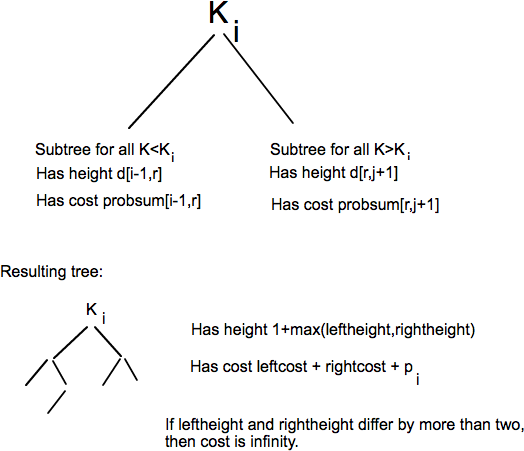
\includegraphics[width=300px]{dyn10.png}
			\label{fig:dyn10}
			\caption{showing the construction of $K_i, \ldots, K_j$ trees}
		\end{figure}
	\newpage
	.
	\newpage
	\noindent
	11.	The input consists of $n$ intervals over the real line. The output should be a collection $C$  of nonoverlapping 
			intervals such the sum of the lengths of the intervals in $C$ is maximized. Give a polynomial
			time algorithm for this problem.\\
			\\
			\\
		  Assume C is sorted such that $C[i].start < C[i+1].start, ~\forall~i$.\\
		  The two-dimensional Lookup[i][j] table stores the maximum length-sum
		  over the line segment between i and j.\\
		  The calculation for Lookup[4,12], for example, is the maximum of:\\
		  Lookup[4,5] + Lookup[5,12]\\
		  Lookup[4,6] + Lookup[6,12]\\
		  \vdots\\
		  Lookup[4,11] + Lookup[11,12].\\
			\\
			\begin{verbatim}
			  // Initialization
			  start = inf
			  end = 0
			  For i = 1 to n:
			    Lookup[i,i] = 0
			    Lookup[C[i].start, C[i].end] = C[i].end - C[i].start
			    start = min(start, C[i].start)
			    end = max(end, C[i].end)
			  
			  For i = start to end:
			    For j = i to start:
			      If Lookup[i,j] is not set (not initialized):
			        max = 0
			        For x = i+1 to j-1:
			          If Lookup[i,x] + Lookup[x,j] > max:
			            max = Lookup[i,x] + Lookup[x,j]
			            
			            // store which cells compose the max
			            Lookup[i,j].children = Lookup[i,x], Lookup[x,j] 
			        Lookup[i,j] = max
			\end{verbatim}
			\\
			The maximum length for this problem is found at Lookup[start][end]. What 
			segments make up this length can be determined by Lookup[start][end].children.
			Repeat the procedure until the initialized nodes are found (those without children). 
			% answer here
\end{document}